% Figura Anexo I: STIGLITZ-WEISS: el rendimiento del banco tiene joroba y el crédito se raciona en equilibrio
\documentclass[tikz,border=3pt]{standalone}
\usepackage[T1]{fontenc}
\usepackage[utf8]{inputenc}
\usepackage{amsmath}
\usetikzlibrary{arrows.meta,calc,positioning}
\begin{document}
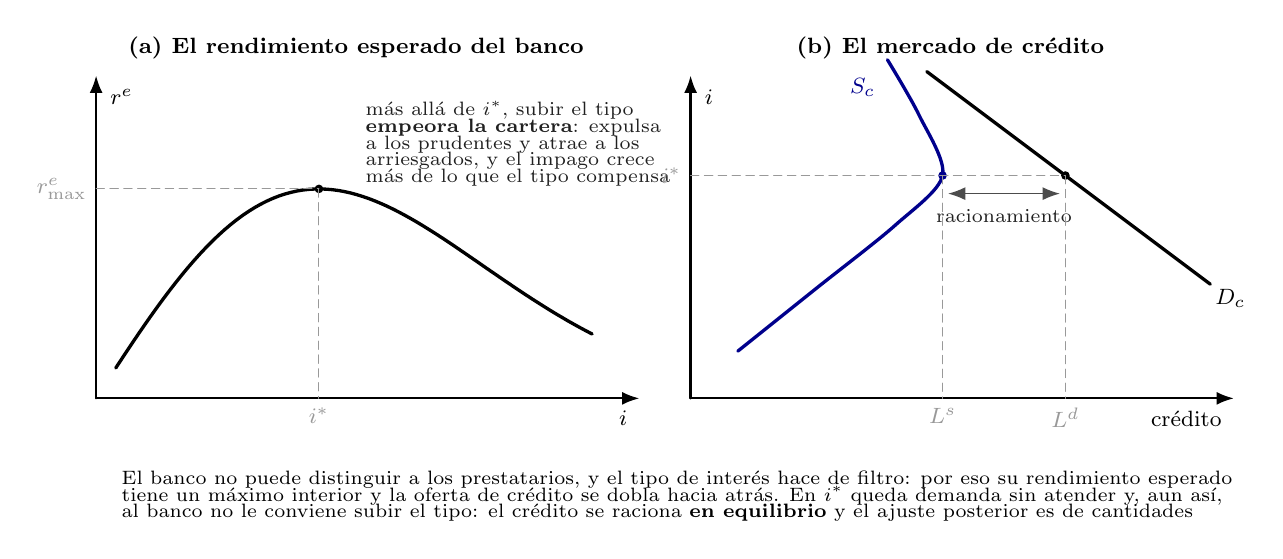
\begin{tikzpicture}[>={Latex[length=2.2mm]}, line cap=round, font=\footnotesize,
  eje/.style={->, thick},
  curva/.style={very thick},
  nueva/.style={very thick, blue!55!black},
  guia/.style={densely dashed, gray!80},
  pto/.style={circle, fill=black, inner sep=1.1pt}]
  % ---------- Panel (a): rendimiento esperado del banco ----------
  \node[font=\footnotesize\bfseries] at (3.3,4.45) {(a) El rendimiento esperado del banco};
  \draw[eje] (0,0) -- (6.9,0) node[below left=1pt]{$i$};
  \draw[eje] (0,0) -- (0,4.1) node[below right=2pt]{$r^{e}$};
  \draw[curva, domain=0.25:6.3, samples=80] plot (\x,{1.55*\x*exp(-(\x/4)^2)});
  \node[pto] (M) at (2.83,2.66) {};
  \draw[guia] (2.83,2.66) -- (2.83,0) node[below]{$i^{*}$};
  \draw[guia] (0,2.66) node[left]{$r^{e}_{\max}$} -- (2.83,2.66);
  \node[align=left, anchor=north west, font=\scriptsize, gray!25!black] at (3.3,3.9)
    {más allá de $i^{*}$, subir el tipo\\[-2pt]\textbf{empeora la cartera}: expulsa\\[-2pt]a los prudentes y atrae a los\\[-2pt]arriesgados, y el impago crece\\[-2pt]más de lo que el tipo compensa};
  % ---------- Panel (b): el mercado con racionamiento ----------
  \begin{scope}[xshift=7.55cm]
    \node[font=\footnotesize\bfseries] at (3.3,4.45) {(b) El mercado de crédito};
    \draw[eje] (0,0) -- (6.9,0) node[below left=1pt]{crédito};
    \draw[eje] (0,0) -- (0,4.1) node[below right=2pt]{$i$};
    % Demanda: i = 6.4 - 0.75 L
    \draw[curva] (3.0,4.15) -- (6.6,1.45) node[below right=-3pt]{$D_c$};
    % Oferta doblada hacia atras
    \draw[nueva] plot [smooth] coordinates {(0.6,0.6) (1.6,1.4) (2.6,2.2) (3.2,2.83) (2.9,3.6) (2.5,4.3)};
    \node[anchor=east, inner sep=2pt, blue!55!black] at (2.42,3.95) {$S_c$};
    \node[pto, fill=blue!55!black] (S) at (3.2,2.83) {};
    \node[pto] (Dp) at (4.76,2.83) {};
    \draw[guia] (0,2.83) node[left]{$i^{*}$} -- (4.76,2.83);
    \draw[<->, gray!60!black, shorten >=2pt, shorten <=2pt] (3.2,2.6) -- (4.76,2.6);
    \node[font=\scriptsize, anchor=north, text=gray!25!black] at (3.98,2.52) {racionamiento};
    \draw[guia] (3.2,2.83) -- (3.2,0) node[below]{$L^{s}$};
    \draw[guia] (4.76,2.83) -- (4.76,0) node[below]{$L^{d}$};
  \end{scope}
  \node[align=left, anchor=north west, font=\scriptsize] at (0.2,-0.8)
    {El banco no puede distinguir a los prestatarios, y el tipo de interés hace de filtro: por eso su rendimiento esperado\\[-2pt]tiene un máximo interior y la oferta de crédito se dobla hacia atrás. En $i^{*}$ queda demanda sin atender y, aun así,\\[-2pt]al banco no le conviene subir el tipo: el crédito se raciona \textbf{en equilibrio} y el ajuste posterior es de cantidades};
\end{tikzpicture}
\end{document}
